\documentclass[border=10]{standalone}
\usepackage{tikz}
\usetikzlibrary{shapes.multipart}
\usetikzlibrary{shapes,arrows}
\usetikzlibrary{arrows.meta,positioning}
\usetikzlibrary{fadings}

\begin{document}

\begin{frame}
  \centering
  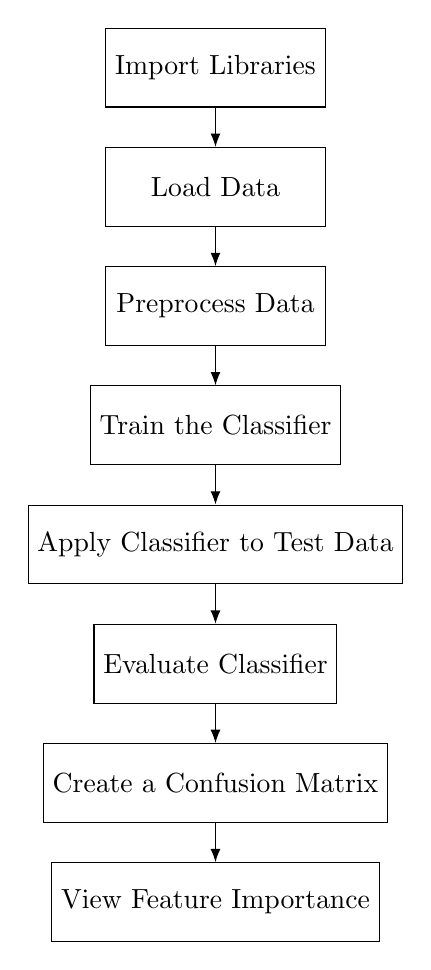
\begin{tikzpicture}[node distance=5mm, >=Latex,
    block/.style = {draw, rectangle, minimum height=10mm, minimum width=28mm,align=center},]
    \node [block] (prelim) {Import Libraries};
    \node [block, below=of prelim] (load_data) {Load Data};
    \node [block, below=of load_data] (preproc_data) {Preprocess Data};
    \node [block, below=of preproc_data] (train) {Train the Classifier};
    \node [block, below=of train] (apply) {Apply Classifier to Test Data};
    \node [block, below=of apply] (eval_classify) {Evaluate Classifier};
    \node [block, below=of eval_classify] (conf_matrix) {Create a Confusion Matrix};
    \node [block, below=of conf_matrix] (feat_imp) {View Feature Importance};
    \draw[->] (prelim) edge (load_data);
    \draw[->] (load_data) edge (preproc_data);
    \draw[->] (preproc_data) edge (train);
    \draw[->] (train) edge (apply);
    \draw[->] (apply) edge (eval_classify);
    \draw[->] (eval_classify) edge (conf_matrix);
    \draw[->] (conf_matrix) edge (feat_imp);
  \end{tikzpicture}
\end{frame}

\end{document}